% !TEX root = ../main.tex

\chapter{Creativity}
\label{ch:creativity}

\emph{Part of this research has been described in a journal article in Digital Creativity in 2013, and I presented a paper at the Creativity and Cognition conference 2013 in Sydney.}

\grule{}

\todo{finish intro to creativity and computers chapter}

Educational psychologist Richard Mayer identified several different approaches to human creativity research and each approach has its own methodologies and goals. \citep[p.453]{Mayer1999}

\begin{description}
  \item [Psychometric] (creativity as a mental trait): quantitative measurement, controlled environments, ability based analysis
  \item [Psychological] (creativity as cognitive processing): controlled environments, quantitative measurements, cognitive task analysis
  \item [Biographical] (creativity as a life story): authentic environments, qualitative descriptions, quantitative measurements
  \item [Biological] (creativity as a physiological trait): physiological measures
  \item [Computational] (creativity as a mental computation): formal modelling
  \item [Contextual] (creativity as a context-based activity): social, cultural and evolutionary context
\end{description}

There are many debates across the involved disciplines. Specifically, Mayer identified five big questions of human creativity research: \citep[p.450-451]{Mayer1999}

\begin{enumerate}
  \item Is creativity a property of people, products, or processes?
  \item Is creativity a personal or social phenomenon?
  \item Is creativity common or rare?
  \item Is creativity domain-general or domain-specific?
  \item Is creativity quantitative or qualitative?
\end{enumerate}

\begin{quote}
  An important challenge for the next 50 years of creativity research is to develop a clearer definition of creativity and to use a combination of research methodologies that will move the field from speculation to specification. \citep[p.459]{Mayer1999}
\end{quote}

\begin{quote}
  ``In research communities, approaches to the study of creativity differ in three main respects: 1$)$ the type of research design, whether experimental, psychometric, observational etc. 2$)$ the focus of the research, whether on human attributes cognitive processes or features of creative outcomes, and 3$)$ the type of information that is used for the basis of evidence, by which is meant whether the time frame is present (real-time observation) or past (historical data) and whether the situation is artificial (laboratory) or natural (real world settings).'' \citep[p.3]{Candy2012}% chktex 10
\end{quote}

Creativity is a human quality --- a process\marginpar{process}. Computers are essentially a product of human creativity\marginpar{product}.

Models of human creativity don't necessarily apply to computer creativity.

Creativity can be studied at various \textbf{levels} (neurological, cognitive, and holistic/systemic), from different \textbf{perspectives} (subjective and objective) and \textbf{characteristics} (combinational, exploratory and transformative).

This chapter introduces relevant models of human and computer creativity and describes the disciplines of computational creativity and creative computing.

\begin{draft}
  These two simple statements already point to one of the main problems with evaluating creative computer software: do we evaluate the process or the product? See §~\ref{ch:interpretation}.
\end{draft}

\todo{put summaries at back of chapter or front? styling?}

\clearpage

\vspace*{\fill}

\begin{shaded}
  Summary:
  \begin{itemize}
    \item novelty/typicality/acceptability/variety/imagination/originality
    \item quality/value/appreciation/appropriateness/usefulness/relevance (/surprising?)
    \item efficiency/skill
    \item subjective/P/little-c
    \item objective/H/Big-C
    \item combinational, exploratory and transformative
    \item product/process
    \item The 4 P’s
    \item Unified theory
    \item Associative and bisociative thinking
    \item Creative triptych (humour, discovery, art)
    \item 4 step model
    \item Problem solving
    \item P-creativity and H-creativity
  \end{itemize}
\end{shaded}

\clearpage


\section{In Humans}

\todo{general introduction about human creativity models}

Let us define creativity as \emph{the ability to use original ideas to create something new and surprising of value}. We generally speak of creative ideas rather than products, since creative products merely provide evidence of a creative process that has already taken place.

\begin{quote}
  ``Creativity is the interaction among aptitude, process, and environment by which an individual or group produces a perceptible product that is both novel and useful as defined within a social context'' (Plucker et al., 2004, p. 90) \citep{Jordanous2012}
\end{quote}


\subsection{Mel Rhodes and Ross Mooney}

Mel Rhodes (1916--1976), who has a background in education and psychology, identified four common themes of creativity in 1961, which he termed ``the four P’s of creativity'' \citep{Rhodes1961}:

\begin{description}
  \item [Persons] personality, intellect, temperament, physique, traits, habits, attitudes, self-concept, value systems, defence mechanisms and behaviour.
  \item [Process] motivation, perception, learning, thinking and communication.
  \item [Press] relationship between human beings and their environment
  \item [Products] a thought which has been communicated to other people in the form of words, paint, clay, metal, stone, fabric, or other material.
\end{description}

Rhodes highlights the importance of a holistic view on creativity through these four areas of study, which he hoped would become the basis of a unified theory of creativity.

\begin{draft}
  Where, what, who and how – those are the questions we need to ask regarding creativity.
\end{draft}

Ross Mooney identified four aspects of creativity in 1963 (as cited in \citep{Sternberg1999}) which are essentially the same.

\begin{enumerate}
  \item The creative environment
  \item The creative person
  \item The creative process
  \item The creative product
\end{enumerate}

\todo{Mel Rhodes vs Ross Mooney??}

\begin{draft}
  I believe these four aspects represent four conditions of creativity in a way, since all of them influence the outcome. Sometimes the creative environment and the creative person are merged into one, simply because people are often a product of their environment. The person will always be influenced by its surroundings, its culture, family, etc.\ and the environment alone cannot influence anything if not through a person. Another interpretation of course is that the creative environment is the context in which the creative product exists. Depending on which way we look at it, the first and second can be interchanged. This project focuses on the creative product, making sure the essence of the search tool is creative – the algorithms that define the main functionality of the search tool.
\end{draft}

\begin{figure}[htb] % (here, top, bottom, page)
  \centering
  \tikzset{every fit/.append style=text badly centered}
  \tikzset{class/.style={draw,rectangle},
           label/.style={align=center,inner ysep=2pt,outer ysep=2pt,node distance=4pt}}
  \begin{tikzpicture}
  \node [class] (prod) {Product};
  \node [label, below=of prod] (proc) {Process};
  \node [label, below=of proc] (pers) {Person};
  \node [label, below=of pers] (env) {Environment};
  \begin{pgfonlayer}{background}
  \node [class, inner xsep=1em, fit=(prod) (proc)] {};
  \node [class, inner xsep=2em, fit=(prod) (proc) (pers)] {};
  \node [class, inner xsep=2em, fit=(prod) (proc) (pers) (env)] {};
  \end{pgfonlayer}
  \end{tikzpicture}
\caption[4 Aspects of Creativity]{4 Aspects of Creativity}
\label{fig:4Crea}
\end{figure}

\begin{draft}
  Figure~\ref{fig:4Crea} shows how these aspects relate to each other. The environment influences all others and the person creates the product in a process.
\end{draft}


\subsection{Arthur Koestler}

Arthur Koestler (1905--1983) published his study on creativity entitled ``The Act of Creation'' in 1964 \citep{Koestler1964}. The book still carries influence today. His main contribution to the field is probably the concept of \gls{bisociation}, a term he coined for the idea of two ``self-consistent but habitually incompatible frames of reference'' intersecting to give rise to new creative idea \citep[p.35]{Koestler1964}. It is interesting however to look at some of his other views on creativity as well.

He splits creativity into three domains, a triptych, without sharp boundaries: humour, discovery and art (see table~\ref{KHDA}). All creative acts traverse the three domains of this triptych from left to right, that is, the emotional climate of the creator changes ``from an absurd through an abstract to a tragic or lyric view of existence'' during the process \citep[p.27]{Koestler1964}. Central to all three domains is the ``discovery of hidden similarities'', or bisociation. Koestler differentiates between associative thinking and bisociative thinking. He links those broadly to habit and originality, respectively. More specifically, associative thinking is conscious, logical, habitual, rigid, repetitive and conservative and bisociative thinking is unconscious, intuitive, original, flexible, novel and destructive/constructive.

% \begin{table}[p]
%   \centering
%   \begin{tabu}{cc}
%   \toprule
%   \textbf{Associative} & \textbf{Bisociative}     \\
%   \midrule
%   Conscious            & Unconscious              \\
%   Logic                & Intuition                \\
%   Habit                & Originality              \\
%   Rigid                & Flexible                 \\
%   Repetitive           & Novel                    \\
%   Conservative         & Destructive/Constructive \\
%   \bottomrule
%   \end{tabu}
% \caption[Associative vs Bisociative]{Koestler: Associative vs Bisociative}
% \label{KAB}
% \end{table}

\begin{table}[htbp]
  \centering
  \begin{tabu}{ccccc}
  \toprule
  \textbf{Humour}
  &
  $\Rightarrow$
  &
  \textbf{Discovery}
  &
  $\Rightarrow$
  &
  \textbf{Art}
  \\
  \midrule
  Laugh           && Understand         && Marvel       \\
  Riddle          && Problem            && Allusion     \\
  Debunking       && Discovering        && Revealing    \\
  Coincidence     && Trigger            && Fate         \\
  Aggressive      && Neutral            && Sympathetic  \\
  \bottomrule
  \end{tabu}
\caption[Creative Triptych]{Koestler: Creative Triptych}
\label{KHDA}
\end{table}


\subsection{Henri Poincaré, Graham Wallas and George Pólya}

Henri Poincaré (1854--1912) \citep{Poincare2001} and Graham Wallas (1858--1932) \citep{Wallas1926} have defined a popular model \citep{Boden2003, Koestler1964, Partridge1994} of the creative process (it was suggested by Poincaré  (\citep{Poincare2001} book: ``science and method'', chapter III:\@``mathematical discovery'', pages 387--400) and formulated by Wallas).

\begin{enumerate}
  \item Preparation – focusing the mind on the problem
  \item Incubation – unconscious internalising
  \item Illumination – eureka moment from unconsciousness to consciousness
  \item Verification – conscious evaluation of the idea and elaboration…
\end{enumerate}

Weisberg criticises the stages of incubation and illumination \citep[referred to by][]{Partridge1994}, saying that the creative process is really just simple problem solving, and that incubation is what he calls ``creative worrying''.

\begin{quote}
  ``First, we have to \textbf{understand} the problem; we have to see clearly what is required. Second, we have to see how the various items are connected, how the unknown is linked to the data, in order to obtain the idea of the solution, to make a \textbf{plan}. Third, we \textbf{carry out} our plan. Fourth, we \textbf{look back} at the completed solution, we review and discuss it.'' \citep[p.5-6, his emphasis]{Polya1957}
\end{quote}


\subsection{James Kaufman and Ron Beghetto}

\todo{DOB of authors?}
James C. Kaufman (1974-) and Ronald A. Beghetto (DOB?)\ldots\citep[See][]{Kaufman2009}.

\begin{figure}[htb] % (here, top, bottom, page)
  \centering
  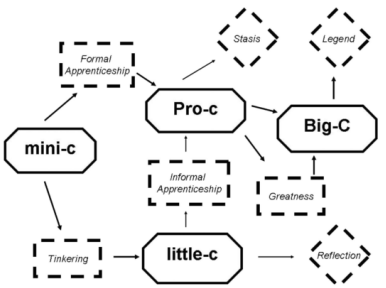
\includegraphics[width=\linewidth]{images/4C.png}
\caption[The 4 C Model]{The 4 C Model}
\label{fig:4C}
\end{figure}

\todo{redo diagram}

\tikzstyle{format} = [draw, thin, fill=blue!20]
\tikzstyle{medium} = [ellipse, draw, thin, fill=green!20, minimum height=2.5em]
\begin{figure}[htbp]
  \centering
  \framebox{
\begin{tikzpicture}[node distance=3cm, auto,>=latex', thick]
    % We need to set at bounding box first. Otherwise the diagram
    % will change position for each frame.
    \path[use as bounding box] (-1,-4) rectangle (10,2); %(-1,0) rectangle (10,-2);
    \path[->] node[format] (tex) {Pro-c};
    \path[->] node[format, right of=tex] (dvi) {Big-C}
                  (tex) edge node {\TeX} (dvi);
    \path[->] node[format, right of=dvi] (ps) {mini-c}
                  node[medium, below of=dvi] (screen) {screen}
                  (dvi) edge node {dvips} (ps)
                        edge node[swap] {xdvi} (screen);
    \path[->] node[format, right of=ps] (pdf) {little-c}
                  node[medium, below of=ps] (print) {printer}
                  (ps) edge node {ps2pdf} (pdf)
                       edge node[swap] {gs} (screen)
                       edge (print);
    \path[->] (pdf) edge (screen)
                        edge (print);
    \path[->, draw] (tex) -- +(0,1) -| node[near start] {pdf\TeX} (pdf);
\end{tikzpicture}
}
\caption[The 4 C Model2]{The 4 C Model2}
\label{fig:4C2}
\end{figure}

\begin{description}
  \item [Big-C] Eminent Accomplishments. Big-C creativity consists of clear-cut, eminent creative contributions. Big-C creativity often requires a degree of time. Indeed, most theoretical conceptions of Big-C nearly require a posthumous evaluation.
  \item [Pro-c] Professional Expertise. Pro-c represents the developmental and effortful progression beyond little-c. The concept of Pro-c is consistent with the expertise acquisition approach of creativity. \todo{ref}\textbf{Ericsson1996, Ericsson2007} Propulsion Theory of Creative Contributions \citep{Sternberg1999, Sternberg2006}: Replication, redefinition, forward incrementation, advance forward incrementation. Redirection, Reconstruction, reinitation, integration.
  \item [Little-c] Everyday Innovation. More focused on everyday activities, such as those creative actions in which the non-expert may participate each day.
  \item [Mini-c] Transformative Learning. Encompasses the creativity inherent in the learning process. ``Mini-c is defined as the novel and personally meaningful interpretation of experiences, actions, and events.'' \citep{Beghetto2007} Central to the definition of mini-c creativity is the dynamic, interpretive process of constructing personal knowledge and understanding within a particular sociocultural context. ``a transformation or reorganization of incoming information and mental structures based on the individual's characteristics and existing knowledge'' \textbf{[p.63]Moran2003}\todo{ref} Moreover, mini-c stresses that mental constructions that have not (yet) been expressed in a tangible way can still be considered highly creative. Mini-c highlights the intrapersonal, and more process focused aspects of creativity.
\end{description}

Applies to all: openness to new experiences, active observation, and willingness to be surprised and explore the unknown.


\subsection{Margaret Boden}

Professor Margaret Boden (1936-) is a prominent figure in the fields of \gls{cc} and computational creativity. She has a background in medical sciences, psychology and philosophy and currently works as a cognitive scientist in computer science and artificial intelligence. Her main interest is in how the human mind works and how computer models of the mind and specific thinking processes can help us understand both better. She has provided two important contributions to the field. The first is her description of three distinct forms of creativity and the second is her important distinction between two senses of creativity \citep{Boden2003}.

\begin{quote}
  [Creativity is] the ability to come up with ideas or artefacts that are \textbf{new, surprising and valuable}. \citep{Boden2003} (her emphasis).
\end{quote}

She identified three distinct forms or cognitive processes of how creativity can happen. These are combinational, exploratory and transformational creativity, which can happen at the same time. \citep{Boden2003}[17, 21].

\begin{description}
  \item [Combinational creativity] making unfamiliar combinations of familiar ideas; juxtaposition of dissimilar; bisociation; deconceptualisation
  \item [Exploratory creativity] exploration of conceptual spaces; noticing new things in old spaces
  \item [Transformative creativity] transformation of space; making new thoughts possible by altering the rules of old conceptual space
\end{description}

Central to these three forms is the idea of a \textbf{conceptual space}. For any idea, its conceptual space describes the characteristics and constraints that define it in its most fundamental way. The conceptual space of a tea cup would contain information like: it is a container that can hold a hot fluid, it should hold about a half a pint of fluid and it might or might not be built in such a way as to not burn the hand that carries it. The specific colour of the cup or what material it is made of for example are not contained in its conceptual space.

Combinational creativity is the most common form of the three and is concerned with the unusual juxtaposition of common ideas. This aspect is highlighted in her definition of creativity, which requires novelty and surprise. The main idea is that any particular combination of ideas has to be unusual, causing surprise, but not (necessarily) the individual ideas themselves. She safeguards against purely random combination by including the usefulness of the result as a requirement in the definition. Exploratory creativity requires a person (or computer program) to fully explore the conceptual space of an idea and find unusual or interesting aspects of it. This form of creativity is about pushing an idea to its limits. Transformational creativity takes this exploration one step further. Once the limits of an idea have been identified, they can be transformed. This means that we can step out of the normal conceptual space of an idea, create a new one, alter or ignore the given constraints, add new ones, etcetera.

Boden argues that creative ideas are surprising because they go against expectations \citep{Boden2003}. She also believes that constraints support creativity and are even essential for it to happen.

\begin{quote}
  Constraints map out a territory of structural possibilities which can then be explored, and perhaps transformed to give another one. \citep{Boden2003}
\end{quote}

These three forms of creativity can be then interpreted on two levels. Any idea should be viewed and evaluated at the appropriate level. Consider the following scenario. A child and a professional architect both build a corbelled arch out of material available to them. Who is being creative here? The level of expertise is clearly different between the two. The child has no experience and is experimenting with the possibilities and limitations of the building blocks (exploring their conceptual space) while the architect has studied the technique for years and is simply applying knowledge he has learned from others (familiar use of a familiar idea). Clearly the child is being more creative in this example. Boden proposed to view and judge the creativity of these two persons separately by differentiating between two levels of creativity, a personal one and a historical one. \textbf{Psychological creativity} (P-creativity) is a personal kind of creativity that is novel in respect to an individual and \textbf{historical creativity} (H-creativity) is fundamentally novel in respect to the whole of human history. The child in the earlier scenario was P-creative but the architect was neither, he was simply applying his trained skills.

\begin{quote}
	P–creativity involves coming up with a surprising, valuable idea that’s new to the person who comes up with it. It doesn’t matter how many people have had that idea before. But if a new idea is H–creative, that means that (so far as we know) no one else has had it before: it has arisen for the first time in human history. \citep{Boden2003}
\end{quote}

\begin{quote}
  Boden suggests that it is helpful to regard aspects such as novelty, quality and process as dimensions of creativity. Instead of asking ‘is x creative?’ (assuming a boolean judgement) or ‘how creative is x?’ (assuming a linear judgement) we should ask ‘where does x lie in creativity space?’ (assuming an n-dimensional space for n criteria where we can measure each dimension). \citep[p.8]{Pease2001}
\end{quote}

\begin{quote}
  Boden argues that process does matter, stating that a program is creative only if it produces items in the right way --- by transforming the boundaries of a conceptual space. This, she claims, can only be done if the program contains reflexive descriptions which mark its own procedures and is capable of varying them. The program should contain a meta-level which assesses methods of transforming a space and considers when and how to apply them. \citep[p.8]{Pease2001}
\end{quote}


\subsection{Robert J. Sternberg, James C. Kaufman and Timothy Leary}

Sternberg and Kaufman identify a set of personality traits that are associated with creative people in their ``Handbook of Creativity'' \citep{Sternberg1999, Sternberg1999}. These are independence of judgement, self-confidence, and attraction to complexity, aesthetic orientation, and tolerance for ambiguity, openness to experience, psychoticism, risk taking, androgyny, perfectionism, persistence, resilience, and self-efficacy. It is easy to find common characteristics among creative people but that doesn't mean that these automatically make a person or a product they make creative.

Timothy Leary took this idea of common characteristics a bit further and suggested there are four types of creative personalities ([25] as cited in [27]).\todo{ref} From his ideas we can draw the conclusion that a creative person needs to be able to make novel combinations from novel ideas.

\begin{description}
  \item [Reproductive Blocked] (no novel combinations, no direct experience)
  \item [Reproductive Creator] (no direct experience, but crafty skill in producing new combinations of old symbols)
  \item [Creative Creator] (new experience presented in novel performances)
  \item [Creative Blocked] (new direct experience expressed in conventional modes)
\end{description}

Tables~\ref{Leary1} and~\ref{Leary2} are in Leary's words.

\begin{table}[htbp]
  \everyrow{\hrule}
  \tabulinesep = 2mm % chktex 1
  \begin{tabu}{|X|X|X|X|}
  \textbf{Reproductive Blocked}
  &
  \textbf{Reproductive Creator}
  &
  \textbf{Creative Creator}
  &
  \textbf{Creative Blocked}
  \\
  The routine, well-socialised person who experiences only in terms of what he has been taught and who produces only what has been produced before.
  &
  The innovating performer who experiences only in terms of the available categories but has learned to manipulate these categories in novel combinations.
  &
  The person who experiences directly outside the limits of ego and labels, and who has learned to develop new models of communications, or who can manipulate familiar categories in novel combinations or who can let natural modes develop under his nurture.
  &
  The person who experiences uniquely and sensitively outside of game concepts (either by choice or helplessly by inability) but who is unable to communicate or uninterested in communicating these experiences outside the conventional manner.
  \\
  Reproductive Performer
  &
  \multicolumn{2}{c|}{Creative Performer}
  &
  Reproductive Performer
  \\
  \multicolumn{2}{|c|}{Reproductive Experience}
  &
  \multicolumn{2}{c|}{Creative Experience}
  \\
  \end{tabu}
\caption[Leary's four types of creativity]{Leary's four types of creativity}
\label{Leary1}
\end{table}

\begin{table}[htbp]
  \everyrow{\hrule}
  \tabulinesep = 2mm % chktex 1
  \begin{tabu}{|X|X|X|X|}
  \textbf{Reproductive Blocked}
  &
  \textbf{Reproductive Creator}
  &
  \textbf{Creative Creator}
  &
  \textbf{Creative Blocked}
  \\
  Unimaginative, incompetent hack.
  &
  Reliable nihilist, insensitive, unsuccessful innovator whose shock value changes to morbid curiosity as fads of performance change.
  &
  The mad creative genius, the undiscovered far-out crackpot creator who is recognised by later generations as a creative giant.
  &
  Psychotic, religious crank, eccentric who uses conventional forms for expressing mystical convictions.
  \\
  Competent, responsible, reliable worker.
  &
  Bold initiator who wins game recognitions but whose fame crumbles as fads of performance change.
  &
  The truly creative giant recognised by his own age and the ages to come.
  &
  Solid, reliable person with a ``deep streak''.
  \\
  Reproductive Performer
  &
  \multicolumn{2}{c|}{Creative Performer}
  &
  Reproductive Performer
  \\
  \multicolumn{2}{|c|}{Reproductive Experience}
  &
  \multicolumn{2}{c|}{Creative Experience}
  \\
  \end{tabu}
\caption[Leary's Social Labels]{Leary's social labels to describe the types of creativity}
\label{Leary2}
\end{table}


\section{In Computers}

In this section I am summarising a few models that try to implement creative thinking models in computers. It is really just a survey of different concepts and views and does not immediately apply to my specific research on creative search tools unfortunately.


\subsection{Bipin Indurkhya}

Indurkhya argues that there are two main cognitive mechanisms of creativity: namely juxtaposition of dissimilar and deconceptualization. He says that we are constraint by associations of our concept networks that we inherit and learn in our lifetime, but that computers do not have those conceptual associations and have therefore an advantage when it comes to creative thinking \citep{Indurkhya}. He suggests a computer model using two layers that interact with each other: a perceptual and a conceptual layer.

\begin{itemize}
  \item Juxtaposition of dissimilar
  \item Deconceptualization
\end{itemize}


\subsection{Partridge and Rowe}

Partridge and Rowe have written a good survey of computational models of creativity in their book ``Computers and Creativity'' \citep{Partridge1994} although it is now probably quite out of date (the book was published in 1994). They mention the computer as an unbiased medium for executing creative programs \citep[p.26]{Partridge1994}. Some of the computational methodologies they discuss are as follows, many taken from classical artificial intelligence research.

\begin{itemize}
  \item Generative  grammars
  \item Discovery programs
  \item Rule based systems
  \item Meta-rules (which reason about and create new rules)
  \item Analogical mechanisms
  \item Flexible representations
  \item Classifier systems
  \item Decentralised systems
  \item Connectionist systems
  \item Neural networks
  \item Emergent memory models
\end{itemize}

Classifier systems for example, consist of a set of rules and a message list.

\begin{enumerate}
  \item Place input messages on current message list
  \item Find all rules that can match messages
  \item Each such rule generates a message for the new message list
  \item Replace current message list with the new one
  \item Process new list for any system output
  \item Return to step 1
\end{enumerate}

These can easily be combined with genetic algorithms to enable the system to learn an appropriate classifier set. This is called emergent behavior. Another approach is connectionism a.k.a.\ neural networks. They then go on to describe their emergent-memory model. They are applying the ideas of Poincare and Wallas and are heavily influence by Minsky's theory of K-lines \citep{Minsky1980, Minsky1988}. They define the following characteristics for creative programs:

\begin{itemize}
  \item flexible knowledge representation scheme
  \item representational imprecision
  \item multiple representations
  \item self-assessment
  \item full elaboration
\end{itemize}


\subsection{David Gelernter}

Gelernter introduces a theory of how the human mind works in \citep{Gelernter1994}. His ``spectrum model'' is based on the idea of mental focus and relates well to creativity. According to him we have a thought spectrum. The higher the mental focus, the more awake we are, the more adult we are and modern, logical and rational, convergent, abstract and detailed. The less focused we are the younger or ancient or dreaming we are. Low focus thoughts are metaphoric, hallucinations, divergent, creative, inspirations, concrete, ambient and emotional. Emotions glue low focus thoughts together.

He gives a good example of his own computer program that is being trained by a set of simple pairs (or memories) in the form -mood: happy- for example. These sets of pairs form the experience of the system, the memory that the system can access. It's fetching all memory pairs that match a certain probe, then generalizes them and picks out a feature that is common to all and then uses that to probe further if necessary.

He models his spectrum concept in a way that if we want the system to operate at low focus, more memory pairs would be fetched and more generalised features are deducted and so on. He describes his FGP program (Fetch Generalise Project) as follows \citep[p.132]{Gelernter1994}.

\begin{enumerate}
  \item Fetch memory pairs in response to a probe (question)
  \item Sandwhich them together and peer through the bundle at once
  \item Notice the common features that emerge strongly (generalise)
  \item Pick out interesting emergent details and probe further if necessary
\end{enumerate}

With low focus the system would not generalise as much and just pick out a particular memory, etc. The computer system he has built seems very limited. His memory pairs cannot describe everything. For example they can describe states but not actions.

This idea of accessing thoughts/memories is very closely related to searching. Searching an index in a search engine is similar to remembering, trying to find all memories related to the current thought for example.


\subsection{Marvin Minsky}

Minsky introduces the concepts of k-lines in his Society of Mind \citep{Minsky1980, Minsky1988}. It is basically a theory of memory. He claims that the ``function of a memory is to recreate a state of mind''. His theory of k-lines is as follows.

\begin{quote}
  When you get an idea, or solve a problem, or have a memorable experience, you create what we shall call a K-line. This K-line gets connected to those mental agencies that were actively involved in the memorable mental event. When that K-line is later activated, it reactivates some of those mental agencies, creating a partial mental state resembling the original. \citep{Minsky1980, Minsky1988}
\end{quote}

This theory works quite well with Gelernter's idea of memory. K-lines in this sense are nothing other than Gelernter's memory pairs.

He and his student Push Singh have formalised the idea of a panalogy, which could be relevant for my project. The idea is that an idea can and should be conceptualised in many different ways. This could be seen as a fall-back mechanism for computational models, if one approach didn't return the desired/expected results.


\subsection{Matthew Elton}

Elton explains the concept of ``Artificial Creativity'' which can be seen as a sub-area of \gls{ai}. \gls{ai} research isn't human enough, he argues, it needs to include less abstract ideas like emotions, morals, aesthetic sensibility and creativity. He goes on to explain in detail how production, evaluation and etiology play a role in everything \citep{Elton1995}.

Opposed to the tradidtional approach of \gls{ai} to study  some aspect of the human brain in a specific domain only, he argues that in order to understand creativity we need to look at more than that. Creativtiy arises from a process that is not isolated. The etiology (its history) is essential for something to be classed as creative. Generation (of artefacts or ideas) cannot count as creative if it doesn't undergo evaluation in the process. In order to evaluate we need a sound knowledge of the relevant domain. ``We want creative evaluation to be influenced by a longstanding history of interaction with entities (of whatever kind) in the world.'' Computer systems can be seen in two perspectives: plastic and implastic (resettable). ``All systems can be seen from the implastic perspective since ultimately all systems are built out of physical components that are (statically) well behaved, but for certain explanatory purposes some are best understood plastically.'' Connectionist networks are an example of a plastic system. The brain is a plastic system too.

How do we get enough cultural information and background into the machine to train it? ``There is no pure science of creativity, because it is paradigmatically idiographic --- it can only be understood against the backdrop of a particular history.''

His comments on evaluation are inspirational. How do I make my system evaluate its results or productions (as opposed to me testing my system)?


\section{In Academia}

Two transdisciplinary fields of study have emerged from the variety of disciplines concerned. These are computational creativity and creative computing. The former lies at the cross section of artificial intelligence and cognitive science and the latter is mostly distinguished by its involvement in art. Creative computing focuses on the process of creativity rather than just the outcome as in computational creativity.

\begin{shaded}
  Summary\\
  •	Boden: Combinational, exploratory and transformative \citep{Boden2003, Wiggins2006} (process)\\
  •	Boden: new, surprising, valuable \citep{Boden2003} (product)\\
  •	Colton: Skill + appreciation + imagination = creativity (or the appearance of) \citep{Colton2008a} (product+process)\\
  •	Wiggins: relevance + acceptatbility + quality \citep{Wiggins2006} (product)\\
  •	Ritchie: typicality + quality \citep{Ritchie2001, Ritchie2007} (product)\\
  •	Pease: novelty + value \citep{Pease2001} (product+process)\\
  •	Ventura: efficiency + variety \citep{Ventura2008} (product+process)\\
  •	Jordanious: value (related concepts: usefulness, appropriateness, relevance) + novelty (related concepts: originality, newness) \citep{Jordanous2012}
\end{shaded}

\todo{references}

The concept of creative computing has existed for some time but has not yet managed to evolve into a recognised discipline within computer science. Computational creativity, on the other hand, has emerged as a field within artificial intelligence research\footnote{\url{http://www.computationalcreativity.net/iccc2013/}} and overlaps with creative computing ideas to some extent.

It is important to differentiate between the terms creative computing and computational creativity. Intuitively the former is about doing computations in a creative way, while the latter is about achieving creativity through computation. You can think of the latter falling into the artificial intelligence category (using formal computational methods to mimic creativity as a human trait, see also\footnote{\url{http://www.computationalcreativity.net/iccc2013/}}) and the former being a more poetic endeavour of how the computing itself is done, no matter what the actual purpose of the program is.

As a good example of creative computing, consider the International Obfuscated C Code Contest\footnote{\url{http://www.ioccc.org/}}. The competition revolves around writing compilable/runnable code, while visually appearing as obfuscated as possible. They value unusuality, obscurity and creativity but expect contestants to follow the strict rules and constraints of the C programming language.

Examples of computational creativity are Simon Colton's Painting Fool\footnote{\url{http://www.thepaintingfool.com/}} or Harold Cohen's AARON\footnote{\url{http://www.kurzweilcyberart.com/aaron/history.html}}; both are computer programs that paint pictures. Kurzweil's Cybernetic Poet\footnote{\url{http://www.kurzweilcyberart.com/poetry/rkcp_overview.php}} is a classic example of a program that produces poetry.

But how may we apply the insights into creativity described above in computing? One approach is described by Simon Colton \citep{Colton2008}, who suggests we should adopt human skill, appreciation and imagination.

\begin{quote}
  Without skill, they would never produce anything. Without appreciation, they would produce things which looked awful. Without imagination, everything they produced would look the same. \citep{Colton2008}
\end{quote}

He thinks that evaluating the worth of an idea or product is the biggest challenge facing computational creativity. Whereas in conventional problem solving success is defined as finding a solution, in a creative context more aesthetic considerations have to be taken into account. He suggests three ways for computer programs to generate creative artefacts:

\begin{enumerate}
  \item Mimicking human skill
  \item Mimicking human appreciation
  \item Mimicking human imagination
\end{enumerate}


\subsection{Computational Creativity}

Computational creativity is a relatively new discipline and as such not well defined. Simon Colton, the creator of the Painting Fool, describes it as the discipline of generating artefacts of real value to someone \citep{Colton2008}. This is in contrast to classic artificial intelligence problem solving. He identifies that evaluating the worth of such an artefact as the biggest problem of computational creativity. In problem solving, success is when a solution to the problem has been found. In artefact generation a more aesthetic consideration has to be taken into account.

\begin{draft}
  One could say that computational creativity is the attempt at giving computers the skills, appreciation and imagination needed to produce creative artefacts. Whether or not this makes the computer creative or the programmer is another question that I will not try to answer here.
\end{draft}

Computational creativity has emerged from within \gls{ai} research. Simon Colton and Geraint Wiggins argue \gls{ai} falls within a problem solving paradigm: ``an intelligent task, that we desire to automate, is formulated as a particular type of problem to be solved '' \citep[p.2]{Colton2012}, whereas ``in Computational Creativity research, we prefer to work within an artefact generation paradigm, where the automation of an intelligent task is seen as an opportunity to produce something of cultural value. '' \citep[p.2, my emphasis]{Colton2012}

The International Association for Computational Creativity (ACC)  promotes the advancement of computational creativity which is defined as follows.

\begin{quote}
  Computational Creativity is the art, science, philosophy and engineering of computational systems which, by taking on particular responsibilities, exhibit behaviours that unbiased observers would deem to be creative. (\gls{iccc}14 website)
\end{quote}

Computational creativity is multidisciplinary, bringing together researchers from artificial intelligence, cognitive psychology, philosophy, and the arts. Its role within computer science falls under the scientific paradigm \citep[p.8]{Hugill2013}, \citep[see also][]{Eden2007}, as opposed to \gls{cc} in the technocratic paradigm. Its main goal is to model, simulate or replicate human creativity using a computer and it has the following three aims:

\begin{itemize}
  \item to construct a program or computer capable of human-level creativity
  \item to better understand human creativity and to formulate an algorithmic perspective on creative behavior in humans
  \item to design programs that can enhance human creativity without necessarily being creative themselves
\end{itemize}

The ACC manages the annual \gls{iccc}, whose recent call for papers  (for \gls{iccc} 2014) gives a useful insight into their research agenda. It can be broken down as follows:

\begin{itemize}
  \item Paradigms, metrics, frameworks, formalisms, methodologies, perspectives
  \item Computational creativity-support tools
  \item Creativity-oriented computing in education
  \item Domain-specific vs.\ generalised creativity
  \item Process vs.\ product
  \item Domain advancement vs.\ creativity advancement
  \item Black box vs.\ accountable systems
\end{itemize}

Simon Colton and Geraint Wiggins have also identified several directions for future research in the field: \citep[p.5]{Colton2012}

\begin{enumerate}
  \item Continued integration of systems to increase their creative potential.
  \item Usage of web resources as source material and conceptual inspiration for creative acts by computer.
  \item Using crowd sourcing and collaborative creative technologies bringing together evaluation methodologies based on product, process, intentionality and the framing of creative acts by software.
\end{enumerate}

\begin{draft}
  This reminds of the 4 P’s, and \gls{cc} and \gls{dh} models
\end{draft}

\begin{shaded}
  \begin{itemize}
  \item Domain-specific vs.\ generalised creativity
  \item Process vs.\ product
  \item Domain advancement vs.\ creativity advancement
  \item Black box vs.\ accountable systems
  \end{itemize}
\end{shaded}


\subsection{Creative Computing}

\todo{rewrite and format}

In the recent first issue of the \gls{ijcrc} Hugill and Yang introduced \gls{cc} as a new discipline \citep{Hugill2013c} with an overarching theme of ``unite and conquer'' \citep[p.1, his emphasis]{Yang2013}. Its broad aim is to ``reconcile the objective precision of computer systems (mathesis) with the subjective ambiguity of human creativity (aesthesis).'' \citep[p.5]{Hugill2013c}. Hugill and Yang suggest \gls{cc} falls within the technocratic paradigm of computing \citep[see also][p.8]{Eden2007}, i.e.\ the discipline is closest related to software engineering, rather than mathematics or natural sciences. They identify five main topics for \gls{cc} research \citep[p.15-17]{Hugill2013c}:

\begin{description}
  \item [Challenges] transdisciplinarity, cross-compatibility, continuity and adaptivity
  \item [Types] creative development of a product, development of a \gls{cc} product and development of tool for creativity support
  \item [Mechanisms]	Boden’s combinational, exploratory and transformational creativity
  \item [Methods] development of suitable transdisciplinary \gls{cc} research methodologies
  \item [Standards] resist standardisation, novel, continuous user interaction, creative mechanisms
\end{description}

The main challenge is for technology  to become ``more adaptive, smarter and better engineered to cope with frequent changes of direction, inconsistencies, irrelevancies, messiness and all the other vagaries that characterise the creative process'' \citep[p.5]{Hugill2013c}. In part, these issues are due to the transdisciplinary nature of the field and factors such as common semantics, standards, requirements and expectations are typical challenges. Hugill and Yang therefore argue that creative software should be flexible and able to adapt to ever changing requirements, it should be evaluated and re-written continuously and it should be cross-compatible.

The different \textbf{types} of \gls{cc} highlight the different aspects researcher and practitioners focus on during their work. These are

\begin{description}
  \item [Process]  creative development of a computing product,
  \item [Product] development of a Creative Computing product and
  \item [Community] development of computing environment to support creativity.
\end{description}

The creative computing process should consist of combinational, exploratory and transformational activities (in the sense of Margaret Boden’s theory, as discussed in \todo{cross ref}).

\begin{draft}
  Broadly speaking, you could say that approaches to \gls{cc} are therefore either bottom-up (1) or top-down (2).
\end{draft}

The third type of \gls{cc} in a way reflects what Hugill and Yang call the ``local and global levels'', which represent the two types of creativity identified by Boden (P- and H-creativity, see above). It is concerned with developing environments, tools and methods and the management of these.

\begin{draft}
  This includes cross-compatibilty, which directly represents the solution to the personal/local and historical/global issues mentioned by Boden and Hugill and Yang.
\end{draft}

Similar to the four step model of the creative process by Poincaré and Wallas \citep{Poincare2001, Wallas1926} and the four step model of problem solving by Pólya \citep{Polya1957}, they propose a four step model for the creative computing process. They do this by comparing the acts of artistic creation and software engineering in some detail. They found that the two processes follow essentially the same levels of abstraction (from the abstract to the concrete). The four steps are \citep[p.15]{Hugill2013c}:

\begin{enumerate}
  \item Motivation (digitised thinking)
  \item Ideation (design sketch)
  \item Implementation (creative system)
  \item Operation (effect of system/revision)
\end{enumerate}

\begin{draft}
  This reminds of the 4 P’s, and \gls{cc} and \gls{dh} models??
\end{draft}

% \begin{table}[htbp]
%   \centering
%   \begin{tabu}{cc}
%   \toprule
%   \textbf{Associative} & \textbf{Bisociative}     \\
%   \midrule
%   Conscious            & Unconscious              \\
%   Logic                & Intuition                \\
%   Habit                & Originality              \\
%   Rigid                & Flexible                 \\
%   Repetitive           & Novel                    \\
%   Conservative         & Destructive/Constructive \\
%   \bottomrule
%   \end{tabu}
% \caption[Associative vs Bisociative]{Koestler: Associative vs Bisociative}
% \label{KAB}
% \end{table}

Given the transdisciplinary nature of \gls{cc}, Hugill and Yang suggest that existing research methodologies are unsuitable and new ones have to be developed. The following is an example of a possible \gls{cc} research methodology they propose as a starting point \citep[p.17]{Hugill2013c}:

\begin{enumerate}
  \item Review literature across disciplines
  \item Identify key creative activities
  \item Analyse the processes of creation
  \item Propose approaches to support these activities and processes
  \item Design and implement software following this approach
  \item Experiment with the resulting system and propose framework
\end{enumerate}

Hugill and Yang propose four \textbf{standards} for \gls{cc} \citep[p.17]{Hugill2013c} namely, resist standardisation, perpetual novelty, continuous user interaction and combinational, exploratory and or transformational.

\begin{shaded}
  Summary\\
  •	Transdisciplinary\\
  •	Technocratic paradigm of computer science\\
  •	Mathesis + aesthesis\\
  •	Local + global\\
  •	Top-down + bottom-up\\
  •	Continuous life-cycle, cross-compatibility, adaptive software, interoperability
\end{shaded}


\subsection{Speculative Computing}

SpecLab \citep{Drucker2009} is a book by Johanna Drucker about her experiences as a researcher moving between disciplines and the projects she worked on as part of the Digital Humanities laboratory at the University of Virginia, USA\@. Several of those had pataphyscial inspirations.

In his review, on the back cover of the book, John Unsworth says that Drucker ``emphasizes the graphical over the textual, the generative over the descriptive, and aesthetic subjectivity over analytical objectivism.'' Her main argument is that in the design of digital knowledge representation, subjectivity and aesthetics are an essential feature. She confronts logical computation with aesthetic principles with the idea that design is information.

Aesthesis is the theory of ambiguous and subjective knowledge, ideological and epistemological, while Mathesis is formal objective logic and they contrast each other. Knowledge is always interpretation and subjectivity is always in opposition to objectivity. Knowledge becomes synonymous with information and as such can be represented digitally as data and metadata.

\begin{quote}
  Arguably, few other textual forms will have greater impact on the way we read, receive, search, access, use and engage with the primary materials of humanities studies than the metadata structures that organize and present that knowledge in digital form. \citep[p.9]{Drucker2009}
\end{quote}

But how is this metadata analysed? How do we analyse this type of structured data? And most important of all she asks, what can be considered as data, what can be expressed in those quantitative terms or other standard parameters? Is data neutral, raw or does it have meaning? Here she also points out that many information structures have graphical analogies and can be understood as diagrams that organize the relations of elements within the whole.

Because ``computational methods rooted in formal logic tend to be granted more authority […] than methods grounded in subjective judgement'', she introduces the discipline of Speculative Computing as the solution to that problem.  The concept can be understood as a criticism of mechanistic, logical approaches that distinguish between subject and object.

\begin{quote}
  Speculative computing takes seriously the destabilization of all categories of entity, identity, object, subject, interactivity, process, or instrument. In short, it rejects mechanistic, instrumental, and formally logical approaches, replacing them with concepts of autopoiesis (contingent interdependency), quantum poetics and emergent systems, heteroglossia, indeterminacy and potentiality, intersubjectivity, and deformance. Digital Humanities is focused on texts, images, meanings, and means. Speculative Computing engages with interpretation and aesthetic provocation. \citep[p.29]{Drucker2009}
\end{quote}

Pataphysics governs exceptions and anomalies and she introduces a, what she calls, ``patacritical'' method of including those exceptions as rules --- even if repeatability and reliability are compromised. Bugs and Glitches are privileged over functionality, and although that may not be as useful in all circumstances, they are ``valuable to speculation in a substantive, not trivial, sense.'' In an essay on speculative computing \citep{Drucker2007} she says ``Pataphysics celebrates the idiosyncratic and particular within the world of phenomena, thus providing a framework for an aesthetics of specificity within generative practice.'' To break out of the formal logic and defined parameters of computer science we need speculative capabilities and Pataphysics. ``The goal of pataphysical and speculative computing is to keep digital humanities from falling into mere technical application of standard practices.''

\begin{quote}
  ``'Pataphysics inverts the scientific method, proceeding from and sustaining exceptions and unique cases, while quantum methods insist on conditions of indeterminacy as that which is intervened in any interpretative act. Dynamic and productive with respect to the subject-object dialectic of perception and cognition, the quantum extensions of speculative aesthetics have implications for applied and theoretical dimensions of computational humanities.'' \citep{Drucker2007}% chktex 34
\end{quote}

With this, Drucker introduces Speculative Aesthetics, which links interface design in which other speculative computing principles. She also refers to Kant and his idea of ``purposiveness without purpose.'' She says that the appreaciation of design as it is (outside of untility) is the goal of speculative aesthetics.


\subsection{Digital Humanities}

Anne Burdick, Johanna Drucker, Peter Lunefeld, Todd Presner and Jeffrey Schnapp (referred to as `the authors' in this section) have collaboratively written an authoritative manifesto for the field of \gls{dh} \citep{Burdick2012}. Computing has had a big impact on the humanities as a discipline so much so that \gls{dh} was born of the encounter between the two \citep[p.3]{Burdick2012}. In essence, it is characterised by \textbf{collaboration, transdisciplinarity and an engagement with computing} \citep[p.122]{Burdick2012} but it should not simply be reduced to doing the humanities digitally \citep[p.101]{Burdick2012}. It spans across many traditional areas of research, such as literature, philosophy, history, art, music, design and of course computer science.

\begin{draft}
  Transliteracy\footnote{Sue Thomas et al.\ define transliteracy as ``the ability to read, write and interact across a range of platforms, tools and media from signing and orality through handwriting, print, TV, radio and film, to digital social networks.'' \citep{Thomas2007}} therefore is fundamental \citep{Thomas2007};
\end{draft}

``The field of Digital Humanities may see the emergence of polymaths who can `do it all'\,'': who can research, write, shoot, edit, code, model, design, network, and dialogue with users. \citep[p.15]{Burdick2012} \gls{dh} encompasses several core activities which on various levels depend on and support each other.

\begin{description}
  \item [Design] Shape, scheme, inform, experience, position, narrate,
  					interpret, remap/reframe, reveal, deconstruct, reconstruct,
  					situate, critique
  \item [Curation, analysis, editing, modelling] Digitise, classify, describe, metadata, organise, navigate
  \item [Computation, processing] Disambiguate, encode, structure, procedure, index, automate, sort, search, calculate, match
  \item [Networks, infrastructure] Cultural, institutional, technical, compatible, interoperable, flexible, mutable, extensible
  \item [Versioning, prototyping, failures]	Iterate, experiment, take-risks, redefine, beta-test
\end{description}

\begin{draft}
  IF THE STUDY OF ART OR HUMAN CREATIVITY FALLS WITHIN HUMANITIES RESEARCH, THEN COMP CREAT SHOULD FALL WITHIN DIGITAL HUMANITIES, RIGHT, AND USE THE TOOLS AND METHODS AVAILABLE.\@
\end{draft}

\subsubsection*{DESIGN}
The authors suggest that ``for digital humanists, design is a creative practice harnessing cultural, social, economic, and technological constraints in order to bring systems and objects into the world.'' \citep[p.13]{Burdick2012}

In generative mode, these designers shape structural logics, rhetorical schemata, information hierarchies, experiential qualities, cultural positioning, and narrative strategies. When working analytically, their task is to visually interpret, remap or reframe, reveal patterns, deconstruct, reconstruct, situate, and critique. \citep[p.12]{Burdick2012}

\subsubsection*{CURATION, ANALYSIS, EDITING, MODELING}
\begin{quote}
  digital activity: digitization, classification, description and metadata, organization, and navigation. \citep[p.17]{Burdick2012}
\end{quote}

\begin{quote}
  Involving archives, collections, repositories, and other aggregations of materials, CURATION is the selection and organization of materials in an interpretive framework, argument, or exhibit. \citep[p.17]{Burdick2012}
\end{quote}

\begin{quote}
  The parsing of the cultural record in terms of questions of authenticity, origin, transmission, or production is one of the foundation stones of humanistic scholar- ship upon which all other interpretive work depends. But editing is also productive and generative, and it is the suite of rhetorical devices that make a work. Editing is the creative, imaginative activity of making, and as such, design can be also seen as a kind of editing \citep[p.18]{Burdick2012}
\end{quote}

\begin{quote}
  MODELING highlights the notion of content models—shapes of argument expressed in information structures and their design. \citep[p.18]{Burdick2012}
\end{quote}

\subsubsection*{COMPUTATION, PROCESSING}
\begin{quote}
  interpretation is rethought through the encounter with computational methods and [] computational methods are rethought through the encounter with humanistic modes of knowing. \citep[p.103]{Burdick2012}
\end{quote}

\begin{quote}
  Humanists have begun to use programming languages. But they have yet to create programming languages of their own: languages that can come to grips with, for example, such fundamental attributes of cultural communication and traditional objects of humanistic scrutiny as nuance, inflection, undertone, irony, and ambivalence. \citep[p.103]{Burdick2012}
\end{quote}

\begin{figure}[htbp]
  \centering
    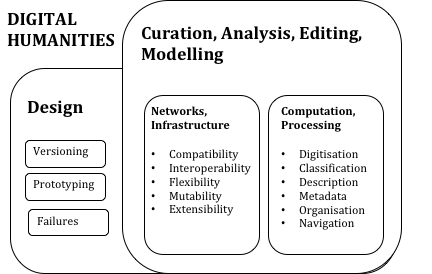
\includegraphics{images/dh01.png}
  \caption[Digital Humanities]{Digital Humanities model}
\label{fig:Digital_Humanities}
\end{figure}

\subsubsection*{NETWORKS, INFRASTRUCTURE}
\begin{quote}
  Designing and building digital projects depend on knowledge of these fundamentals and on a nuanced understanding of the net- worked environments in which the projects will develop and variously reside. \citep[p.17]{Burdick2012}
\end{quote}

\begin{quote}
  Digital work takes place in the real world, and humanists once accus- tomed to isolated or individualized modes of production must now grapple with complex partnerships and with insuring the long-term availability and viability of their scholarship \citep[p.21]{Burdick2012}
\end{quote}

\subsubsection*{VERSIONING, PROTOTYPING, FAILURES}
\begin{quote}
  one of the strongest attributes of the field is that the iterative versioning of digital projects fosters experimentation, risk-taking, redefinition, and sometime failure. \citep[p.21]{Burdick2012}
\end{quote}

\begin{draft}
  SOUNDS LIKE SOFTWARE ENGINEERING
\end{draft}

\begin{quote}
  It is important that we do not short-circuit this experimental process in the rush to normalize practices, standardize methodologies, and define evaluative metrics. \citep[p.21]{Burdick2012}
\end{quote}

\begin{draft}
  argument for creative computing too
\end{draft}

\subsubsection*{Field map of digital humanities: emerging methods and genres}\citep[p.29-60]{Burdick2012}

\begin{alltt}
•	enhanced critical curation
o	digital collections
o	multimedia critical editions
o	object-based argumentation
o	expanded publication
o	experiential and spatial
o	mixed physical and digital
•	augmented editions and fluid textuality
o	structured mark-up
o	natural language processing
o	relational rhetoric
o	textual analysis
o	variants and versions
o	mutability
•	scale: the law of large numbers
o	quantitative analysis
o	text-mining
o	machine reading
o	digital cultural record
o	algorithmic analysis
•	distant/close, macro/micro, surface/depth
o	large-scale patterns
o	fine-grained analysis
o	close reading
o	distant reading
o	differential geographies
•	cultural analytics, aggregation, and data-mining
o	parametrics
o	cultural mash-ups
o	computational processing
o	composite analysis
o	algorithm design
•	visualization and data design
o	data visualization
o	mapping
o	information design
o	simulation environments
o	spatial argument
o	modelling knowledge
o	visual interpretation
•	locative investigation and thick mapping
o	spatial humanities
o	digital cultural mapping
o	interconnected sites
o	experimental navigation
o	geographic information systems (GIS)
o	stacked data
•	the animated archive
o	user communities
o	permeable walls
o	active engagement
o	bottom-up curation
o	multiplied access
o	participatory content creation
•	distributed knowledge production and performative access
o	global networks
o	ambient data
o	collaborative authorship
o	interdisciplinary teams
o	use as performance
o	crowd-sourcing
•	humanities gaming
o	user engagement
o	rule-based play
o	rich interaction
o	virtual learning environments
o	immersion and simulation
o	narrative complexity
•	code, software, and platform studies
o	narrative structures
o	code as text
o	computational processes
o	software in a cultural context
o	encoding practices
•	database documentaries
o	variable experience
o	user-activated
o	multimedia prose
o	modular and combinatoric
o	multilinear
•	repurposable content and remix culture
o	participatory Web
o	read/write/rewrite
o	platform migration
o	sampling and collage
o	meta-medium
o	inter-textuality
•	pervasive infrastructure
o	extensible frameworks
o	heterogeneous data streams
o	polymorphous browsing
o	cloud computing
•	ubiquitous scholarship
o	augmented reality
o	web of things
o	pervasive surveillance and tracking
o	ubiquitous computing
o	deterritorialization of humanistic practice
\end{alltt}

\begin{draft}
  quantifiable and repeatable phenomena versus complex dynamics of interpretation, cultural meanings, probabilistic modelling, interpretive mapping, subjective visualizations, and self-customizing navigation \citep[p.103]{Burdick2012}
\end{draft}

\subsubsection*{TOOLS}
\begin{quote}
  Building tools around core humanities concepts: subjectivity, ambiguity, contingency, observer-dependent variables in the production of knowledge: holds the promise of expanding current models of knowledge. As such, the next generation of digital experimenters could contribute to humanities theory by forging tools that quite literally embody humanities centred views regarding the world. \citep[p.104]{Burdick2012}
\end{quote}

\begin{quote}
  Tools are not just tools. They are cognitive interfaces that presuppose forms of mental and physical discipline and organization. By scripting an action, they produce and transmit knowledge, and, in turn, model a world. \citep[p.105]{Burdick2012}
\end{quote}

\begin{quote}
  For all its potential interest, a humanities-centered computational environment could well end up distancing humanistic work from the mainstream of digital society, either because of its specialized or speculative character, or because the values that inform its architecture are at odds with the needs of business for standardization, quantitative metrics, and disambiguation. \citep[p.105]{Burdick2012}
\end{quote}

\begin{shaded}
Summary\\
•	Collaborative, Transdisciplinary and Computing
\end{shaded}

\subsection{Computer Ethics}

\begin{draft}
  ETHICS\@: PROCESS< PRODUCT< PURPOSE\\
  ROBOT ETHICS\@: similar to 4-p’s of creativity \citep{McBride2013}\\

  it has three actors: Robot engineer, client and user.

  4 approaches:\\
  •	challenge the myth of autonomy\\
  •	Developing practice-based approaches (in context of it purpose and environment)\\
  •	Managing ethical variety\\
  •	A model for human0centred robot ethics\\

  Virtuous robot:\\
  •	Human-centred\\
  •	Man-machine interdependency\\
  •	Practice based (context)\\
  •	Ethical variety
\end{draft}% chktex 17
